% Created by tikzDevice version 0.12.3 on 2020-01-25 19:15:40
% !TEX encoding = UTF-8 Unicode
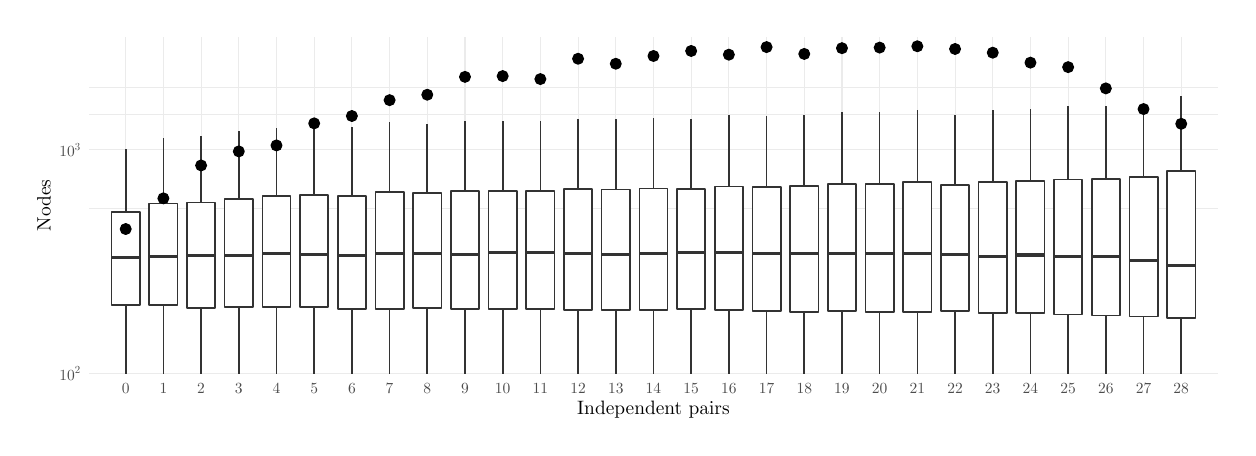
\begin{tikzpicture}[x=1pt,y=1pt]
\definecolor{fillColor}{RGB}{255,255,255}
\path[use as bounding box,fill=fillColor,fill opacity=0.00] (0,0) rectangle (433.62,144.54);
\begin{scope}
\path[clip] ( 22.14, 19.53) rectangle (430.12,141.04);
\definecolor{drawColor}{gray}{0.92}

\path[draw=drawColor,line width= 0.2pt,line join=round] ( 22.14, 79.39) --
	(430.12, 79.39);

\path[draw=drawColor,line width= 0.2pt,line join=round] ( 22.14,113.42) --
	(430.12,113.42);

\path[draw=drawColor,line width= 0.2pt,line join=round] ( 22.14,122.92) --
	(430.12,122.92);

\path[draw=drawColor,line width= 0.4pt,line join=round] ( 22.14, 19.53) --
	(430.12, 19.53);

\path[draw=drawColor,line width= 0.4pt,line join=round] ( 22.14,100.38) --
	(430.12,100.38);

\path[draw=drawColor,line width= 0.4pt,line join=round] ( 35.42, 19.53) --
	( 35.42,141.04);

\path[draw=drawColor,line width= 0.4pt,line join=round] ( 49.04, 19.53) --
	( 49.04,141.04);

\path[draw=drawColor,line width= 0.4pt,line join=round] ( 62.67, 19.53) --
	( 62.67,141.04);

\path[draw=drawColor,line width= 0.4pt,line join=round] ( 76.29, 19.53) --
	( 76.29,141.04);

\path[draw=drawColor,line width= 0.4pt,line join=round] ( 89.91, 19.53) --
	( 89.91,141.04);

\path[draw=drawColor,line width= 0.4pt,line join=round] (103.53, 19.53) --
	(103.53,141.04);

\path[draw=drawColor,line width= 0.4pt,line join=round] (117.15, 19.53) --
	(117.15,141.04);

\path[draw=drawColor,line width= 0.4pt,line join=round] (130.78, 19.53) --
	(130.78,141.04);

\path[draw=drawColor,line width= 0.4pt,line join=round] (144.40, 19.53) --
	(144.40,141.04);

\path[draw=drawColor,line width= 0.4pt,line join=round] (158.02, 19.53) --
	(158.02,141.04);

\path[draw=drawColor,line width= 0.4pt,line join=round] (171.64, 19.53) --
	(171.64,141.04);

\path[draw=drawColor,line width= 0.4pt,line join=round] (185.26, 19.53) --
	(185.26,141.04);

\path[draw=drawColor,line width= 0.4pt,line join=round] (198.89, 19.53) --
	(198.89,141.04);

\path[draw=drawColor,line width= 0.4pt,line join=round] (212.51, 19.53) --
	(212.51,141.04);

\path[draw=drawColor,line width= 0.4pt,line join=round] (226.13, 19.53) --
	(226.13,141.04);

\path[draw=drawColor,line width= 0.4pt,line join=round] (239.75, 19.53) --
	(239.75,141.04);

\path[draw=drawColor,line width= 0.4pt,line join=round] (253.37, 19.53) --
	(253.37,141.04);

\path[draw=drawColor,line width= 0.4pt,line join=round] (267.00, 19.53) --
	(267.00,141.04);

\path[draw=drawColor,line width= 0.4pt,line join=round] (280.62, 19.53) --
	(280.62,141.04);

\path[draw=drawColor,line width= 0.4pt,line join=round] (294.24, 19.53) --
	(294.24,141.04);

\path[draw=drawColor,line width= 0.4pt,line join=round] (307.86, 19.53) --
	(307.86,141.04);

\path[draw=drawColor,line width= 0.4pt,line join=round] (321.48, 19.53) --
	(321.48,141.04);

\path[draw=drawColor,line width= 0.4pt,line join=round] (335.11, 19.53) --
	(335.11,141.04);

\path[draw=drawColor,line width= 0.4pt,line join=round] (348.73, 19.53) --
	(348.73,141.04);

\path[draw=drawColor,line width= 0.4pt,line join=round] (362.35, 19.53) --
	(362.35,141.04);

\path[draw=drawColor,line width= 0.4pt,line join=round] (375.97, 19.53) --
	(375.97,141.04);

\path[draw=drawColor,line width= 0.4pt,line join=round] (389.59, 19.53) --
	(389.59,141.04);

\path[draw=drawColor,line width= 0.4pt,line join=round] (403.22, 19.53) --
	(403.22,141.04);

\path[draw=drawColor,line width= 0.4pt,line join=round] (416.84, 19.53) --
	(416.84,141.04);
\definecolor{drawColor}{gray}{0.20}

\path[draw=drawColor,line width= 0.6pt,line join=round] ( 35.42, 77.89) --
	( 35.42,100.83);

\path[draw=drawColor,line width= 0.6pt,line join=round] ( 35.42, 44.22) --
	( 35.42, 32.09) --
	( 35.42, 13.41) --
	( 35.42,  0.00);
\definecolor{fillColor}{RGB}{255,255,255}

\path[draw=drawColor,line width= 0.6pt,line join=round,line cap=round,fill=fillColor] ( 30.31, 77.89) --
	( 30.31, 44.22) --
	( 35.42, 44.22) --
	( 40.53, 44.22) --
	( 40.53, 77.89) --
	( 35.42, 77.89) --
	( 30.31, 77.89) --
	cycle;

\path[draw=drawColor,line width= 1.1pt,line join=round] ( 30.31, 61.34) --
	( 35.42, 61.34) --
	( 40.53, 61.34);

\path[draw=drawColor,line width= 0.6pt,line join=round] ( 49.04, 80.95) --
	( 49.04,104.79);

\path[draw=drawColor,line width= 0.6pt,line join=round] ( 49.04, 44.22) --
	( 49.04, 25.49) --
	( 49.04,  0.00);

\path[draw=drawColor,line width= 0.6pt,line join=round,line cap=round,fill=fillColor] ( 43.94, 80.95) --
	( 43.94, 44.22) --
	( 49.04, 44.22) --
	( 54.15, 44.22) --
	( 54.15, 80.95) --
	( 49.04, 80.95) --
	( 43.94, 80.95) --
	cycle;

\path[draw=drawColor,line width= 1.1pt,line join=round] ( 43.94, 61.98) --
	( 49.04, 61.98) --
	( 54.15, 61.98);

\path[draw=drawColor,line width= 0.6pt,line join=round] ( 62.67, 81.37) --
	( 62.67,105.47);

\path[draw=drawColor,line width= 0.6pt,line join=round] ( 62.67, 43.33) --
	( 62.67, 23.51) --
	( 62.67,  0.00);

\path[draw=drawColor,line width= 0.6pt,line join=round,line cap=round,fill=fillColor] ( 57.56, 81.37) --
	( 57.56, 43.33) --
	( 62.67, 43.33) --
	( 67.77, 43.33) --
	( 67.77, 81.37) --
	( 62.67, 81.37) --
	( 57.56, 81.37) --
	cycle;

\path[draw=drawColor,line width= 1.1pt,line join=round] ( 57.56, 62.29) --
	( 62.67, 62.29) --
	( 67.77, 62.29);

\path[draw=drawColor,line width= 0.6pt,line join=round] ( 76.29, 82.62) --
	( 76.29,107.07);

\path[draw=drawColor,line width= 0.6pt,line join=round] ( 76.29, 43.51) --
	( 76.29, 24.13) --
	( 76.29,  0.00);

\path[draw=drawColor,line width= 0.6pt,line join=round,line cap=round,fill=fillColor] ( 71.18, 82.62) --
	( 71.18, 43.51) --
	( 76.29, 43.51) --
	( 81.40, 43.51) --
	( 81.40, 82.62) --
	( 76.29, 82.62) --
	( 71.18, 82.62) --
	cycle;

\path[draw=drawColor,line width= 1.1pt,line join=round] ( 71.18, 62.29) --
	( 76.29, 62.29) --
	( 81.40, 62.29);

\path[draw=drawColor,line width= 0.6pt,line join=round] ( 89.91, 83.65) --
	( 89.91,108.35);

\path[draw=drawColor,line width= 0.6pt,line join=round] ( 89.91, 43.51) --
	( 89.91, 24.13) --
	( 89.91,  0.00);

\path[draw=drawColor,line width= 0.6pt,line join=round,line cap=round,fill=fillColor] ( 84.80, 83.65) --
	( 84.80, 43.51) --
	( 89.91, 43.51) --
	( 95.02, 43.51) --
	( 95.02, 83.65) --
	( 89.91, 83.65) --
	( 84.80, 83.65) --
	cycle;

\path[draw=drawColor,line width= 1.1pt,line join=round] ( 84.80, 63.01) --
	( 89.91, 63.01) --
	( 95.02, 63.01);

\path[draw=drawColor,line width= 0.6pt,line join=round] (103.53, 84.04) --
	(103.53,108.80);

\path[draw=drawColor,line width= 0.6pt,line join=round] (103.53, 43.69) --
	(103.53, 23.97) --
	(103.53,  0.00);

\path[draw=drawColor,line width= 0.6pt,line join=round,line cap=round,fill=fillColor] ( 98.42, 84.04) --
	( 98.42, 43.69) --
	(103.53, 43.69) --
	(108.64, 43.69) --
	(108.64, 84.04) --
	(103.53, 84.04) --
	( 98.42, 84.04) --
	cycle;

\path[draw=drawColor,line width= 1.1pt,line join=round] ( 98.42, 62.70) --
	(103.53, 62.70) --
	(108.64, 62.70);

\path[draw=drawColor,line width= 0.6pt,line join=round] (117.15, 83.71) --
	(117.15,108.60);

\path[draw=drawColor,line width= 0.6pt,line join=round] (117.15, 42.80) --
	(117.15, 23.51) --
	(117.15,  0.00);

\path[draw=drawColor,line width= 0.6pt,line join=round,line cap=round,fill=fillColor] (112.05, 83.71) --
	(112.05, 42.80) --
	(117.15, 42.80) --
	(122.26, 42.80) --
	(122.26, 83.71) --
	(117.15, 83.71) --
	(112.05, 83.71) --
	cycle;

\path[draw=drawColor,line width= 1.1pt,line join=round] (112.05, 62.29) --
	(117.15, 62.29) --
	(122.26, 62.29);

\path[draw=drawColor,line width= 0.6pt,line join=round] (130.78, 85.20) --
	(130.78,110.42);

\path[draw=drawColor,line width= 0.6pt,line join=round] (130.78, 42.80) --
	(130.78, 23.82) --
	(130.78,  0.00);

\path[draw=drawColor,line width= 0.6pt,line join=round,line cap=round,fill=fillColor] (125.67, 85.20) --
	(125.67, 42.80) --
	(130.78, 42.80) --
	(135.88, 42.80) --
	(135.88, 85.20) --
	(130.78, 85.20) --
	(125.67, 85.20) --
	cycle;

\path[draw=drawColor,line width= 1.1pt,line join=round] (125.67, 62.81) --
	(130.78, 62.81) --
	(135.88, 62.81);

\path[draw=drawColor,line width= 0.6pt,line join=round] (144.40, 84.71) --
	(144.40,109.70);

\path[draw=drawColor,line width= 0.6pt,line join=round] (144.40, 43.33) --
	(144.40, 24.74) --
	(144.40,  0.00);

\path[draw=drawColor,line width= 0.6pt,line join=round,line cap=round,fill=fillColor] (139.29, 84.71) --
	(139.29, 43.33) --
	(144.40, 43.33) --
	(149.51, 43.33) --
	(149.51, 84.71) --
	(144.40, 84.71) --
	(139.29, 84.71) --
	cycle;

\path[draw=drawColor,line width= 1.1pt,line join=round] (139.29, 62.91) --
	(144.40, 62.91) --
	(149.51, 62.91);

\path[draw=drawColor,line width= 0.6pt,line join=round] (158.02, 85.52) --
	(158.02,110.81);

\path[draw=drawColor,line width= 0.6pt,line join=round] (158.02, 42.80) --
	(158.02, 23.35) --
	(158.02,  0.00);

\path[draw=drawColor,line width= 0.6pt,line join=round,line cap=round,fill=fillColor] (152.91, 85.52) --
	(152.91, 42.80) --
	(158.02, 42.80) --
	(163.13, 42.80) --
	(163.13, 85.52) --
	(158.02, 85.52) --
	(152.91, 85.52) --
	cycle;

\path[draw=drawColor,line width= 1.1pt,line join=round] (152.91, 62.70) --
	(158.02, 62.70) --
	(163.13, 62.70);

\path[draw=drawColor,line width= 0.6pt,line join=round] (171.64, 85.52) --
	(171.64,110.65);

\path[draw=drawColor,line width= 0.6pt,line join=round] (171.64, 42.98) --
	(171.64, 30.84) --
	(171.64, 12.13) --
	(171.64,  0.00);

\path[draw=drawColor,line width= 0.6pt,line join=round,line cap=round,fill=fillColor] (166.53, 85.52) --
	(166.53, 42.98) --
	(171.64, 42.98) --
	(176.75, 42.98) --
	(176.75, 85.52) --
	(171.64, 85.52) --
	(166.53, 85.52) --
	cycle;

\path[draw=drawColor,line width= 1.1pt,line join=round] (166.53, 63.21) --
	(171.64, 63.21) --
	(176.75, 63.21);

\path[draw=drawColor,line width= 0.6pt,line join=round] (185.26, 85.63) --
	(185.26,110.94);

\path[draw=drawColor,line width= 0.6pt,line join=round] (185.26, 42.80) --
	(185.26, 23.82) --
	(185.26,  0.00);

\path[draw=drawColor,line width= 0.6pt,line join=round,line cap=round,fill=fillColor] (180.16, 85.63) --
	(180.16, 42.80) --
	(185.26, 42.80) --
	(190.37, 42.80) --
	(190.37, 85.63) --
	(185.26, 85.63) --
	(180.16, 85.63) --
	cycle;

\path[draw=drawColor,line width= 1.1pt,line join=round] (180.16, 63.21) --
	(185.26, 63.21) --
	(190.37, 63.21);

\path[draw=drawColor,line width= 0.6pt,line join=round] (198.89, 86.17) --
	(198.89,111.64);

\path[draw=drawColor,line width= 0.6pt,line join=round] (198.89, 42.61) --
	(198.89, 23.19) --
	(198.89,  0.00);

\path[draw=drawColor,line width= 0.6pt,line join=round,line cap=round,fill=fillColor] (193.78, 86.17) --
	(193.78, 42.61) --
	(198.89, 42.61) --
	(203.99, 42.61) --
	(203.99, 86.17) --
	(198.89, 86.17) --
	(193.78, 86.17) --
	cycle;

\path[draw=drawColor,line width= 1.1pt,line join=round] (193.78, 62.91) --
	(198.89, 62.91) --
	(203.99, 62.91);

\path[draw=drawColor,line width= 0.6pt,line join=round] (212.51, 86.11) --
	(212.51,111.59);

\path[draw=drawColor,line width= 0.6pt,line join=round] (212.51, 42.43) --
	(212.51, 23.35) --
	(212.51,  0.00);

\path[draw=drawColor,line width= 0.6pt,line join=round,line cap=round,fill=fillColor] (207.40, 86.11) --
	(207.40, 42.43) --
	(212.51, 42.43) --
	(217.62, 42.43) --
	(217.62, 86.11) --
	(212.51, 86.11) --
	(207.40, 86.11) --
	cycle;

\path[draw=drawColor,line width= 1.1pt,line join=round] (207.40, 62.50) --
	(212.51, 62.50) --
	(217.62, 62.50);

\path[draw=drawColor,line width= 0.6pt,line join=round] (226.13, 86.42) --
	(226.13,111.81);

\path[draw=drawColor,line width= 0.6pt,line join=round] (226.13, 42.61) --
	(226.13, 23.82) --
	(226.13,  0.00);

\path[draw=drawColor,line width= 0.6pt,line join=round,line cap=round,fill=fillColor] (221.02, 86.42) --
	(221.02, 42.61) --
	(226.13, 42.61) --
	(231.24, 42.61) --
	(231.24, 86.42) --
	(226.13, 86.42) --
	(221.02, 86.42) --
	cycle;

\path[draw=drawColor,line width= 1.1pt,line join=round] (221.02, 62.91) --
	(226.13, 62.91) --
	(231.24, 62.91);

\path[draw=drawColor,line width= 0.6pt,line join=round] (239.75, 86.32) --
	(239.75,111.71);

\path[draw=drawColor,line width= 0.6pt,line join=round] (239.75, 42.98) --
	(239.75, 24.13) --
	(239.75,  0.00);

\path[draw=drawColor,line width= 0.6pt,line join=round,line cap=round,fill=fillColor] (234.64, 86.32) --
	(234.64, 42.98) --
	(239.75, 42.98) --
	(244.86, 42.98) --
	(244.86, 86.32) --
	(239.75, 86.32) --
	(234.64, 86.32) --
	cycle;

\path[draw=drawColor,line width= 1.1pt,line join=round] (234.64, 63.21) --
	(239.75, 63.21) --
	(244.86, 63.21);

\path[draw=drawColor,line width= 0.6pt,line join=round] (253.37, 87.11) --
	(253.37,112.81);

\path[draw=drawColor,line width= 0.6pt,line join=round] (253.37, 42.43) --
	(253.37, 23.19) --
	(253.37,  0.00);

\path[draw=drawColor,line width= 0.6pt,line join=round,line cap=round,fill=fillColor] (248.27, 87.11) --
	(248.27, 42.43) --
	(253.37, 42.43) --
	(258.48, 42.43) --
	(258.48, 87.11) --
	(253.37, 87.11) --
	(248.27, 87.11) --
	cycle;

\path[draw=drawColor,line width= 1.1pt,line join=round] (248.27, 63.26) --
	(253.37, 63.26) --
	(258.48, 63.26);

\path[draw=drawColor,line width= 0.6pt,line join=round] (267.00, 87.00) --
	(267.00,112.67);

\path[draw=drawColor,line width= 0.6pt,line join=round] (267.00, 42.25) --
	(267.00, 23.82) --
	(267.00,  0.00);

\path[draw=drawColor,line width= 0.6pt,line join=round,line cap=round,fill=fillColor] (261.89, 87.00) --
	(261.89, 42.25) --
	(267.00, 42.25) --
	(272.10, 42.25) --
	(272.10, 87.00) --
	(267.00, 87.00) --
	(261.89, 87.00) --
	cycle;

\path[draw=drawColor,line width= 1.1pt,line join=round] (261.89, 62.91) --
	(267.00, 62.91) --
	(272.10, 62.91);

\path[draw=drawColor,line width= 0.6pt,line join=round] (280.62, 87.31) --
	(280.62,113.16);

\path[draw=drawColor,line width= 0.6pt,line join=round] (280.62, 41.88) --
	(280.62, 22.87) --
	(280.62,  0.00);

\path[draw=drawColor,line width= 0.6pt,line join=round,line cap=round,fill=fillColor] (275.51, 87.31) --
	(275.51, 41.88) --
	(280.62, 41.88) --
	(285.73, 41.88) --
	(285.73, 87.31) --
	(280.62, 87.31) --
	(275.51, 87.31) --
	cycle;

\path[draw=drawColor,line width= 1.1pt,line join=round] (275.51, 62.81) --
	(280.62, 62.81) --
	(285.73, 62.81);

\path[draw=drawColor,line width= 0.6pt,line join=round] (294.24, 88.10) --
	(294.24,113.98);

\path[draw=drawColor,line width= 0.6pt,line join=round] (294.24, 42.25) --
	(294.24, 23.19) --
	(294.24,  0.00);

\path[draw=drawColor,line width= 0.6pt,line join=round,line cap=round,fill=fillColor] (289.13, 88.10) --
	(289.13, 42.25) --
	(294.24, 42.25) --
	(299.35, 42.25) --
	(299.35, 88.10) --
	(294.24, 88.10) --
	(289.13, 88.10) --
	cycle;

\path[draw=drawColor,line width= 1.1pt,line join=round] (289.13, 63.01) --
	(294.24, 63.01) --
	(299.35, 63.01);

\path[draw=drawColor,line width= 0.6pt,line join=round] (307.86, 87.97) --
	(307.86,113.91);

\path[draw=drawColor,line width= 0.6pt,line join=round] (307.86, 41.88) --
	(307.86, 22.39) --
	(307.86,  0.00);

\path[draw=drawColor,line width= 0.6pt,line join=round,line cap=round,fill=fillColor] (302.75, 87.97) --
	(302.75, 41.88) --
	(307.86, 41.88) --
	(312.97, 41.88) --
	(312.97, 87.97) --
	(307.86, 87.97) --
	(302.75, 87.97) --
	cycle;

\path[draw=drawColor,line width= 1.1pt,line join=round] (302.75, 62.81) --
	(307.86, 62.81) --
	(312.97, 62.81);

\path[draw=drawColor,line width= 0.6pt,line join=round] (321.48, 88.70) --
	(321.48,114.80);

\path[draw=drawColor,line width= 0.6pt,line join=round] (321.48, 41.69) --
	(321.48, 22.39) --
	(321.48,  0.00);

\path[draw=drawColor,line width= 0.6pt,line join=round,line cap=round,fill=fillColor] (316.38, 88.70) --
	(316.38, 41.69) --
	(321.48, 41.69) --
	(326.59, 41.69) --
	(326.59, 88.70) --
	(321.48, 88.70) --
	(316.38, 88.70) --
	cycle;

\path[draw=drawColor,line width= 1.1pt,line join=round] (316.38, 62.81) --
	(321.48, 62.81) --
	(326.59, 62.81);

\path[draw=drawColor,line width= 0.6pt,line join=round] (335.11, 87.70) --
	(335.11,113.08);

\path[draw=drawColor,line width= 0.6pt,line join=round] (335.11, 42.06) --
	(335.11, 23.19) --
	(335.11,  0.00);

\path[draw=drawColor,line width= 0.6pt,line join=round,line cap=round,fill=fillColor] (330.00, 87.70) --
	(330.00, 42.06) --
	(335.11, 42.06) --
	(340.21, 42.06) --
	(340.21, 87.70) --
	(335.11, 87.70) --
	(330.00, 87.70) --
	cycle;

\path[draw=drawColor,line width= 1.1pt,line join=round] (330.00, 62.60) --
	(335.11, 62.60) --
	(340.21, 62.60);

\path[draw=drawColor,line width= 0.6pt,line join=round] (348.73, 88.75) --
	(348.73,114.92);

\path[draw=drawColor,line width= 0.6pt,line join=round] (348.73, 41.51) --
	(348.73, 22.55) --
	(348.73,  0.00);

\path[draw=drawColor,line width= 0.6pt,line join=round,line cap=round,fill=fillColor] (343.62, 88.75) --
	(343.62, 41.51) --
	(348.73, 41.51) --
	(353.84, 41.51) --
	(353.84, 88.75) --
	(348.73, 88.75) --
	(343.62, 88.75) --
	cycle;

\path[draw=drawColor,line width= 1.1pt,line join=round] (343.62, 61.98) --
	(348.73, 61.98) --
	(353.84, 61.98);

\path[draw=drawColor,line width= 0.6pt,line join=round] (362.35, 89.04) --
	(362.35,115.15);

\path[draw=drawColor,line width= 0.6pt,line join=round] (362.35, 41.32) --
	(362.35, 22.39) --
	(362.35,  0.00);

\path[draw=drawColor,line width= 0.6pt,line join=round,line cap=round,fill=fillColor] (357.24, 89.04) --
	(357.24, 41.32) --
	(362.35, 41.32) --
	(367.46, 41.32) --
	(367.46, 89.04) --
	(362.35, 89.04) --
	(357.24, 89.04) --
	cycle;

\path[draw=drawColor,line width= 1.1pt,line join=round] (357.24, 62.39) --
	(362.35, 62.39) --
	(367.46, 62.39);

\path[draw=drawColor,line width= 0.6pt,line join=round] (375.97, 89.66) --
	(375.97,116.10);

\path[draw=drawColor,line width= 0.6pt,line join=round] (375.97, 40.94) --
	(375.97, 22.87) --
	(375.97,  0.00);

\path[draw=drawColor,line width= 0.6pt,line join=round,line cap=round,fill=fillColor] (370.86, 89.66) --
	(370.86, 73.15) --
	(370.86, 40.94) --
	(375.97, 40.94) --
	(381.08, 40.94) --
	(381.08, 73.15) --
	(381.08, 89.66) --
	(375.97, 89.66) --
	(370.86, 89.66) --
	cycle;

\path[draw=drawColor,line width= 1.1pt,line join=round] (370.86, 61.98) --
	(375.97, 61.98) --
	(381.08, 61.98);

\path[draw=drawColor,line width= 0.6pt,line join=round] (389.59, 89.81) --
	(389.59,116.33);

\path[draw=drawColor,line width= 0.6pt,line join=round] (389.59, 40.55) --
	(389.59, 21.41) --
	(389.59,  0.00);

\path[draw=drawColor,line width= 0.6pt,line join=round,line cap=round,fill=fillColor] (384.49, 89.81) --
	(384.49, 73.19) --
	(384.49, 40.55) --
	(389.59, 40.55) --
	(394.70, 40.55) --
	(394.70, 73.19) --
	(394.70, 89.81) --
	(389.59, 89.81) --
	(384.49, 89.81) --
	cycle;

\path[draw=drawColor,line width= 1.1pt,line join=round] (384.49, 61.77) --
	(389.59, 61.77) --
	(394.70, 61.77);

\path[draw=drawColor,line width= 0.6pt,line join=round] (403.22, 90.61) --
	(403.22,117.36);

\path[draw=drawColor,line width= 0.6pt,line join=round] (403.22, 40.17) --
	(403.22, 21.57) --
	(403.22,  0.00);

\path[draw=drawColor,line width= 0.6pt,line join=round,line cap=round,fill=fillColor] (398.11, 90.61) --
	(398.11, 73.76) --
	(398.11, 40.17) --
	(403.22, 40.17) --
	(408.32, 40.17) --
	(408.32, 73.76) --
	(408.32, 90.61) --
	(403.22, 90.61) --
	(398.11, 90.61) --
	cycle;

\path[draw=drawColor,line width= 1.1pt,line join=round] (398.11, 60.26) --
	(403.22, 60.26) --
	(408.32, 60.26);

\path[draw=drawColor,line width= 0.6pt,line join=round] (416.84, 92.67) --
	(416.84,119.87);

\path[draw=drawColor,line width= 0.6pt,line join=round] (416.84, 39.58) --
	(416.84, 20.74) --
	(416.84,  0.00);

\path[draw=drawColor,line width= 0.6pt,line join=round,line cap=round,fill=fillColor] (411.73, 92.67) --
	(411.73, 75.33) --
	(411.73, 39.58) --
	(416.84, 39.58) --
	(421.95, 39.58) --
	(421.95, 75.33) --
	(421.95, 92.67) --
	(416.84, 92.67) --
	(411.73, 92.67) --
	cycle;

\path[draw=drawColor,line width= 1.1pt,line join=round] (411.73, 58.57) --
	(416.84, 58.57) --
	(421.95, 58.57);
\definecolor{drawColor}{RGB}{0,0,0}
\definecolor{fillColor}{RGB}{0,0,0}

\path[draw=drawColor,line width= 0.4pt,line join=round,line cap=round,fill=fillColor] ( 35.42, 71.78) circle (  1.96);

\path[draw=drawColor,line width= 0.4pt,line join=round,line cap=round,fill=fillColor] ( 49.04, 82.87) circle (  1.96);

\path[draw=drawColor,line width= 0.4pt,line join=round,line cap=round,fill=fillColor] ( 62.67, 94.76) circle (  1.96);

\path[draw=drawColor,line width= 0.4pt,line join=round,line cap=round,fill=fillColor] ( 76.29, 99.83) circle (  1.96);

\path[draw=drawColor,line width= 0.4pt,line join=round,line cap=round,fill=fillColor] ( 89.91,101.99) circle (  1.96);

\path[draw=drawColor,line width= 0.4pt,line join=round,line cap=round,fill=fillColor] (103.53,109.96) circle (  1.96);

\path[draw=drawColor,line width= 0.4pt,line join=round,line cap=round,fill=fillColor] (117.15,112.62) circle (  1.96);

\path[draw=drawColor,line width= 0.4pt,line join=round,line cap=round,fill=fillColor] (130.78,118.35) circle (  1.96);

\path[draw=drawColor,line width= 0.4pt,line join=round,line cap=round,fill=fillColor] (144.40,120.31) circle (  1.96);

\path[draw=drawColor,line width= 0.4pt,line join=round,line cap=round,fill=fillColor] (158.02,126.76) circle (  1.96);

\path[draw=drawColor,line width= 0.4pt,line join=round,line cap=round,fill=fillColor] (171.64,127.05) circle (  1.96);

\path[draw=drawColor,line width= 0.4pt,line join=round,line cap=round,fill=fillColor] (185.26,125.96) circle (  1.96);

\path[draw=drawColor,line width= 0.4pt,line join=round,line cap=round,fill=fillColor] (198.89,133.31) circle (  1.96);

\path[draw=drawColor,line width= 0.4pt,line join=round,line cap=round,fill=fillColor] (212.51,131.50) circle (  1.96);

\path[draw=drawColor,line width= 0.4pt,line join=round,line cap=round,fill=fillColor] (226.13,134.31) circle (  1.96);

\path[draw=drawColor,line width= 0.4pt,line join=round,line cap=round,fill=fillColor] (239.75,136.12) circle (  1.96);

\path[draw=drawColor,line width= 0.4pt,line join=round,line cap=round,fill=fillColor] (253.37,134.78) circle (  1.96);

\path[draw=drawColor,line width= 0.4pt,line join=round,line cap=round,fill=fillColor] (267.00,137.52) circle (  1.96);

\path[draw=drawColor,line width= 0.4pt,line join=round,line cap=round,fill=fillColor] (280.62,135.05) circle (  1.96);

\path[draw=drawColor,line width= 0.4pt,line join=round,line cap=round,fill=fillColor] (294.24,137.13) circle (  1.96);

\path[draw=drawColor,line width= 0.4pt,line join=round,line cap=round,fill=fillColor] (307.86,137.34) circle (  1.96);

\path[draw=drawColor,line width= 0.4pt,line join=round,line cap=round,fill=fillColor] (321.48,137.82) circle (  1.96);

\path[draw=drawColor,line width= 0.4pt,line join=round,line cap=round,fill=fillColor] (335.11,136.84) circle (  1.96);

\path[draw=drawColor,line width= 0.4pt,line join=round,line cap=round,fill=fillColor] (348.73,135.50) circle (  1.96);

\path[draw=drawColor,line width= 0.4pt,line join=round,line cap=round,fill=fillColor] (362.35,131.90) circle (  1.96);

\path[draw=drawColor,line width= 0.4pt,line join=round,line cap=round,fill=fillColor] (375.97,130.28) circle (  1.96);

\path[draw=drawColor,line width= 0.4pt,line join=round,line cap=round,fill=fillColor] (389.59,122.60) circle (  1.96);

\path[draw=drawColor,line width= 0.4pt,line join=round,line cap=round,fill=fillColor] (403.22,115.13) circle (  1.96);

\path[draw=drawColor,line width= 0.4pt,line join=round,line cap=round,fill=fillColor] (416.84,109.80) circle (  1.96);
\end{scope}
\begin{scope}
\path[clip] (  0.00,  0.00) rectangle (433.62,144.54);
\definecolor{drawColor}{gray}{0.30}

\node[text=drawColor,anchor=base west,inner sep=0pt, outer sep=0pt, scale=  0.56] at ( 11.43, 17.12) {10};

\node[text=drawColor,anchor=base west,inner sep=0pt, outer sep=0pt, scale=  0.39] at ( 17.03, 19.41) {2};

\node[text=drawColor,anchor=base west,inner sep=0pt, outer sep=0pt, scale=  0.56] at ( 11.43, 97.98) {10};

\node[text=drawColor,anchor=base west,inner sep=0pt, outer sep=0pt, scale=  0.39] at ( 17.03,100.27) {3};
\end{scope}
\begin{scope}
\path[clip] (  0.00,  0.00) rectangle (433.62,144.54);
\definecolor{drawColor}{gray}{0.30}

\node[text=drawColor,anchor=base,inner sep=0pt, outer sep=0pt, scale=  0.56] at ( 35.42, 12.52) {0};

\node[text=drawColor,anchor=base,inner sep=0pt, outer sep=0pt, scale=  0.56] at ( 49.04, 12.52) {1};

\node[text=drawColor,anchor=base,inner sep=0pt, outer sep=0pt, scale=  0.56] at ( 62.67, 12.52) {2};

\node[text=drawColor,anchor=base,inner sep=0pt, outer sep=0pt, scale=  0.56] at ( 76.29, 12.52) {3};

\node[text=drawColor,anchor=base,inner sep=0pt, outer sep=0pt, scale=  0.56] at ( 89.91, 12.52) {4};

\node[text=drawColor,anchor=base,inner sep=0pt, outer sep=0pt, scale=  0.56] at (103.53, 12.52) {5};

\node[text=drawColor,anchor=base,inner sep=0pt, outer sep=0pt, scale=  0.56] at (117.15, 12.52) {6};

\node[text=drawColor,anchor=base,inner sep=0pt, outer sep=0pt, scale=  0.56] at (130.78, 12.52) {7};

\node[text=drawColor,anchor=base,inner sep=0pt, outer sep=0pt, scale=  0.56] at (144.40, 12.52) {8};

\node[text=drawColor,anchor=base,inner sep=0pt, outer sep=0pt, scale=  0.56] at (158.02, 12.52) {9};

\node[text=drawColor,anchor=base,inner sep=0pt, outer sep=0pt, scale=  0.56] at (171.64, 12.52) {10};

\node[text=drawColor,anchor=base,inner sep=0pt, outer sep=0pt, scale=  0.56] at (185.26, 12.52) {11};

\node[text=drawColor,anchor=base,inner sep=0pt, outer sep=0pt, scale=  0.56] at (198.89, 12.52) {12};

\node[text=drawColor,anchor=base,inner sep=0pt, outer sep=0pt, scale=  0.56] at (212.51, 12.52) {13};

\node[text=drawColor,anchor=base,inner sep=0pt, outer sep=0pt, scale=  0.56] at (226.13, 12.52) {14};

\node[text=drawColor,anchor=base,inner sep=0pt, outer sep=0pt, scale=  0.56] at (239.75, 12.52) {15};

\node[text=drawColor,anchor=base,inner sep=0pt, outer sep=0pt, scale=  0.56] at (253.37, 12.52) {16};

\node[text=drawColor,anchor=base,inner sep=0pt, outer sep=0pt, scale=  0.56] at (267.00, 12.52) {17};

\node[text=drawColor,anchor=base,inner sep=0pt, outer sep=0pt, scale=  0.56] at (280.62, 12.52) {18};

\node[text=drawColor,anchor=base,inner sep=0pt, outer sep=0pt, scale=  0.56] at (294.24, 12.52) {19};

\node[text=drawColor,anchor=base,inner sep=0pt, outer sep=0pt, scale=  0.56] at (307.86, 12.52) {20};

\node[text=drawColor,anchor=base,inner sep=0pt, outer sep=0pt, scale=  0.56] at (321.48, 12.52) {21};

\node[text=drawColor,anchor=base,inner sep=0pt, outer sep=0pt, scale=  0.56] at (335.11, 12.52) {22};

\node[text=drawColor,anchor=base,inner sep=0pt, outer sep=0pt, scale=  0.56] at (348.73, 12.52) {23};

\node[text=drawColor,anchor=base,inner sep=0pt, outer sep=0pt, scale=  0.56] at (362.35, 12.52) {24};

\node[text=drawColor,anchor=base,inner sep=0pt, outer sep=0pt, scale=  0.56] at (375.97, 12.52) {25};

\node[text=drawColor,anchor=base,inner sep=0pt, outer sep=0pt, scale=  0.56] at (389.59, 12.52) {26};

\node[text=drawColor,anchor=base,inner sep=0pt, outer sep=0pt, scale=  0.56] at (403.22, 12.52) {27};

\node[text=drawColor,anchor=base,inner sep=0pt, outer sep=0pt, scale=  0.56] at (416.84, 12.52) {28};
\end{scope}
\begin{scope}
\path[clip] (  0.00,  0.00) rectangle (433.62,144.54);
\definecolor{drawColor}{RGB}{0,0,0}

\node[text=drawColor,anchor=base,inner sep=0pt, outer sep=0pt, scale=  0.70] at (226.13,  4.86) {Independent pairs};
\end{scope}
\begin{scope}
\path[clip] (  0.00,  0.00) rectangle (433.62,144.54);
\definecolor{drawColor}{RGB}{0,0,0}

\node[text=drawColor,rotate= 90.00,anchor=base,inner sep=0pt, outer sep=0pt, scale=  0.70] at (  8.32, 80.28) {Nodes};
\end{scope}
\end{tikzpicture}
